%%%  Ukázkový text a dokumentace stylu pro text závěrečné (bakalářské a
%%%  diplomové) práce na KI PřF UP v Olomouci
%%%  Copyright (C) 2012 Martin Rotter, <rotter.martinos@gmail.com>
%%%  Copyright (C) 2014 Jan Outrata, <jan.outrata@upol.cz>


%%  Pro získání PDF souboru dokumentu je třeba tento zdrojový text v
%%  LaTeXu přeložit (dvakrát) programem pdfLaTeX.

%%  V případě použití programu BibLaTeX pro tvorbu seznamu literatury
%%  je poté ještě třeba spustit program Biber s parametrem jméno
%%  souboru zdrojového textu bez přípony a následně opět (dvakrát)
%%  přeložit zdrojový text programem pdfLaTeX.

%%  Postup získání Postscriptového souboru je popsán v dokumentaci.


%%  Třída dokumentu implementující styl pro závěrečnou práci. Vybrané
%%  nepovinné parametry (ostatní v dokumentaci):

%%  'master' pro sazbu diplomové práce, jinak se sází bakalářská práce

%%  'field=kód' pro Váš studijní obor, kódy pro diplomovou práci 'uvt'
%%  pro Učitelství výpočetní techniky pro střední školy a 'binf' pro
%%  Bioinformatiku, jinak je výchozí Informatika, a pro bakalářskou
%%  práci 'ainfk' pro Aplikovanou informatiku v kombinované formě,
%%  'inf' pro Informatiku, 'infv' pro Informatiku pro vzdělávání a
%%  'binf' pro Bioinfomatiku, jinak je výchozí Aplikovaná informatika
%%  v prezenční formě

%%  'printversion' pro sazbu verze pro tisk (nebarevné logo a odkazy,
%%  odkazy s uvedením adresy za odkazem, ne odkazy do rejstříku),
%%  jinak verze pro prohlížeč

%%  'biblatex' pro zapnutí podpory pro sazbu bibliografie pomocí
%%  BibLaTeXu, jinak je výchozí sazba v prostředí thebibliography

%%  'language=jazyk' pro jazyk práce, jazyky english pro anglický,
%%  slovak pro slovenský, jinak je výchozí czech pro český

%%  'font=sans' pro bezpatkový font (Iwona Light), jinak výchozí
%%  patkový (Latin Modern)

\documentclass[
%  master,
%  field=inf,
%  printversion,
  biblatex=false,
%  language=english,
  font=serif,
  glossaries=false,
  tables=false,
  theorems=false,
  index
]{kidiplom}

\makeatletter
\newcommand\footnoteref[1]{\protected@xdef\@thefnmark{\ref{#1}}\@footnotemark}
\makeatother


%% Informace pro úvodní strany. V jazyku práce (pokud není v komentáři
%% uvedeno česky) a anglicky. Uveďte všechny, u kterých není v
%% komentáři uvedeno, že jsou volitelné. Při neuvedení se použijí
%% výchozí texty. Text pro jiný než nastavený jazyk práce (nepovinným
%% parametrem language makra \documentclass, výchozí český) se zadává
%% použitím makra s uvedením jazyka jako nepovinného parametru.

%% Název práce, česky a anglicky. Měl by se vysázet na jeden řádek.
\title{Demonstrace práce s datovými strukturami}
\title[english]{Data Structure Demonstration}

%% Volitelný podnázev práce, česky a anglicky. Měl by se vysázet na
%% jeden řádek. Výchozí je prázdný.
%% \subtitle{Demonstrace práce s datovými strukturami}
%% \subtitle[english]{Data Structure Demonstration}

%% Jméno autora práce. Makro nemá nepovinný parametr pro uvedení
%% jazyka.
\author{Patrik Becher}

%% Jméno vedoucího práce (včetně titulů). Makro nemá nepovinný
%% parametr pro uvedení jazyka.
\supervisor{Mgr. Tomáš Kühr, Ph.D.}

%% Volitelný rok odevzdání práce. Výchozí je aktuální (kalendářní)
%% rok. Makro nemá nepovinný parametr pro uvedení jazyka.
%\yearofsubmit{\the\year}

%% Anotace práce, včetně anglické (obvykle překlad z jazyka
%% práce). Jeden odstavec!
\annotation{Cílem bakalářské práce bylo vytvořit nástroj pro podporu výuky algoritmizace, konkrétně práce se základními stromovými datovými strukturami (binární vyhledávací stromy, AVL stromy, červenočerné stromy). Výsledná aplikace podporuje vizualizaci vybraných datových struktur, včetně názorné demonstrace běžně prováděných operací s těmito datovými strukturami se souběžným zobrazením pseudokódu prováděné operace.}

\annotation[english]{Toto mně doplní Míša... :D}

%% Klíčová slova práce, včetně anglických. Oddělená (obvykle) středníkem.
\keywords{Binární vyhledávací stromy, Binární strom, AVL strom, Červenočerný strom, Stromové animace Java, JavaFX}
\keywords[english]{Binary search trees, Binary Tree, AVL tree, Redblack tree, Tree animations, Java, JavaFX}

%% Volitelná specifikace příloh textu práce, i anglicky. Výchozí je '1
%% CD/DVD'.
%\supplements{jedno kulaté placaté CD/DVD s malou kulatou dírou uprostřed}
%\supplements[english]{one round flat CD/DVD with a small round hole in the middle}

%% Poděkování. Stručné!
\thanks{Rád bych poděkoval panu Mgr. Tomáši Kührovi Ph.D. za vedení této bakalářské práce a panu RNDr. Arnoštu Večerkovi za odbornou pomoc a poskytnuté materiály k práci. Dále bych chtěl poděkoval mé rodině a přítelkyni za podporu při tvorbě.}

%% Další dodatečné styly (balíky) potřebné pro sazbu vlastního textu práce.
\usepackage{lipsum}

%% Balíčky pro implementaci seznamů vedle sebe.
\usepackage{amssymb}
\usepackage{enumitem}

%-------------------------------------------------------------
% TODO: Nebylo by špatné barvy a
% zvýraznění syntaxe jazyka GLSL přesunout do
% samostatného souboru.
\usepackage{color}

%-------------------------------------------------------------
% Nadefinuj barvy
\definecolor{backcolour}{rgb}{0.95,0.95,0.92}

%-------------------------------------------------------------
% Nadefinuj zvýraznění syntaxe pro jazyk Pseudo
% TODO: 1) Definice není úplně čistá.
%            2) Přesuň tuto definici do vlastního souboru.
\lstdefinelanguage{Pseudo}
{
  sensitive=false, % keywords are not case-sensitive
  keywords={define, end, return, while, do, if, then, else, elseif, for, to, do, end, relief, paraOcc, loadSample},
  morekeywords={},
  %alsoletter=\#\_, % now I can use # character in keywords
  keywordstyle=\bfseries\color{black}, % style of keywords
  captionpos=b, % Position of the Caption (t for top, b for bottom)
  extendedchars=true, % Allows 256 instead of 128 ASCII characters
  tabsize=2, % number of spaces indented when discovering a tab 
  columns=fixed, % make all characters equal width
  keepspaces=true, % does not ignore spaces to fit width, convert tabs to spaces
  showstringspaces=false, % lets spaces in strings appear as real spaces
  breaklines=true, % wrap lines if they don't fit
  %numbers=left, % show line numbers at the left
  %numberstyle=\ttfamily, % style of the line numbers
  backgroundcolor=\color{backcolour},
  basicstyle=\small\color{black},
  commentstyle=\color{green}, % style of comments
  stringstyle=\color{black}, % style of strings
  morecomment=[l]{//}, % l is for line comment
  morecomment=[s]{/*}{*/}, % s is for start and end delimiter
  morestring=[b]" % defines that strings are enclosed in double quotes
  moredelim=[is][\bfseries]{/@}{@/}
}
%-------------------------------------------------------------

% \noindent pro cely dokument.
% \setlength{\parindent}{0pt}

%-------------------------------------------------------------
\begin{document}
%% Sazba úvodních stran -- titulní, s bibliografickými údaji, s
%% anotací a klíčovými slovy, s poděkováním a prohlášením, s obsahem a
%% se seznamy obrázků, tabulek, vět a zdrojových kódů (pokud jejich
%% sazba není vypnutá).

%-------------------------------------------------------------
% Strany 1 - 6

\maketitle

%% Vlastní text závěrečné práce. Pro povinné závěry, před přílohami,
%% použijte prostředí kiconclusions. Povinná je i příloha s obsahem
%% přiloženého CD/DVD.

%% -------------------------------------------------------------------

%% Zatim neoddelat zjistit co to je.
% \newcommand{\BibLaTeX}{\textsc{Bib}\LaTeX}

%-------------------------------------------------------------
% Strana 7

\section{Úvod}
Tato aplikace vznikla za účelem výuky základních binárních stromů. Obsahuje podporu pro \textit{Binární vyhledávací}, \textit{AVL} a \textit{Červenočerné stromy}. Program pomocí animací zobrazuje operace: \textit{Vyhledávání}, \textit{Vkládání} a \textit{Odebírání} prvků ze stromů. Souběžně s animací zobrazuje stručný pseudokód aktuálně prováděné operace. Dále umožňuje \textit{Opakovat poslední operaci} a \textit{Generování náhodných stromů}.\\

Text samotné práce se dělí na dvě části: \textit{Teoretickou část}, ve které se zabývám teorií vybraných stromů a \textit{Programovou část}, která popisuje samotnou implementaci a funkcionalitu programu.\\

\newpage
\section{Stromy}
V kapitole jsou vysvětleny základní pojmy, které jsou nezbytné k pochopení vlastností \textit{stromů} obsažených v aplikaci. V podkapitolách jsou osvětleny principy pro tvorbu a následnou práci s konkrétními \textit{binárními vyhledávacími stromy}. Využitím těchto principů byl naprogramován tento výukový nástroj.\\

\begin{definition}[Strom]
\textit{Strom} je neorientovaný \footnote{Mezi každými dvěma vrcholy existuje právě jedna cesta.} souvislý \footnote{Vynecháním libovolné hrany vznikne nesouvislý graf.} graf bez kružnic \footnote{Přidáním jakékoli hrany vznikne graf s kružnicí.} \cite{belohlavekALM}.
\end{definition}
\begin{figure}[h!]
\centering
	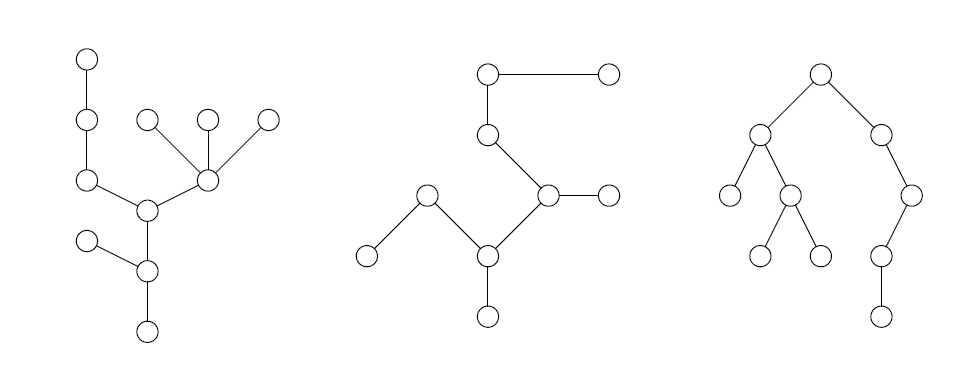
\includegraphics[scale=0.6]{obrazky/1Stromy.png}
	\caption{Příklady neorientovaných stromů}
\end{figure}

\medskip
Strom je datová struktura, která představuje stromovou strukturu propojených \textit{uzlů} \footnote{Prvek obsahující hodnotu.}. Uzly jsou mezi sebou vzájemně spojeny pomocí \textit{hran} \footnote{Představuje cestu mezi spojenými uzly.}. Strom složený z uzlů $U$ má $|U - 1|$ hran.


\begin{definition}[Kořenový strom]
\textit{Kořenový strom} je strom, ve kterém je vybrán jeden vrchol (kořen). Může to být kterýkoliv vrchol. Bývá to ale vrchol, který je v nějakém smyslu na vrcholu hierarchie objektů, která je stromem reprezentována.
\cite{belohlavekALM}
\end{definition}
\smallskip

\newpage
\noindent \textbf{Důležité pojmy:}
\begin{itemize}
\item \textbf{Uzel} -- Jednoduše jakýkoliv prvek stromu.
\item \textbf{Kořen} -- Jeden konkrétní uzel, který se nachází na vrcholu stromu. Pouze tento uzel nemá \textit{rodiče}. 
\item \textbf{Potomek, následník} -- Uzel, který je hranou přímo připojen k jinému uzlu, cestou od kořene.
\item \textbf{Rodič, předchůdce} -- Uzel, který má alespoň jednoho potomka.
\item \textbf{Sourozenci} -- Skupina uzlů, které mají stejného rodiče.
\item \textbf{Podstrom} -- Část stromu, která je úplným stromem, s tím, že kořen tohoto podstromu má svého rodiče.
\item \textbf{Koncový uzel, list} -- Uzel bez potomků. 
\item \textbf{Výška stromu} -- Nejdelší délka cesty od kořene k uzlu.
\end{itemize} 

\begin{figure}[h!]
\centering
	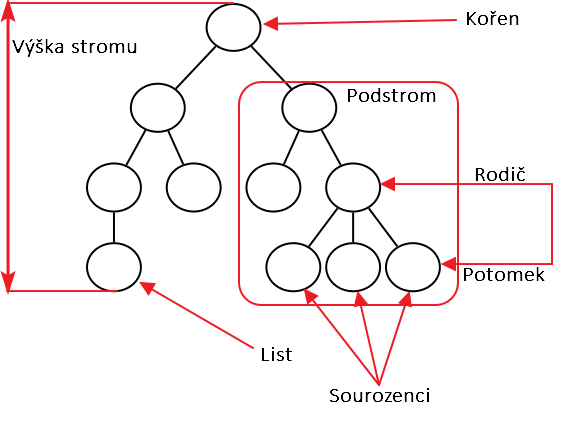
\includegraphics[scale=0.6]{obrazky/2PopisStromu.png}
	\caption{Popis stromu}
\end{figure}

\begin{definition}[$m$-ární stromy]
Kořenový strom se nazývá $m$\textit{-ární}, právě když každý jeho vrchol má nejvýše $m$ potomků. 2-ární strom se nazývá binární. Kořenový strom se nazývá úplný $m$\textit{-ární}, právě když každý jeho vrchol nemá buď žádného nebo má právě $m$ potomků.\cite{belohlavekVychodil}
\end{definition}
\smallskip

\subsection{Binární strom}
\begin{definition}[Binární strom]
\textit{Binární strom} je typ kořenových stromů, ve kterém každý obsažený uzel má maximálně 2 potomky.
\end{definition}
\smallskip

\noindent\textbf{Každý uzel obsahuje tyto vlastnosti:}
\begin{itemize}
\item \textbf{Klíč} -- Hodnota uložená v uzlu.
\item \textbf{Ukazatel na levého potomka.}
\item \textbf{Ukazatel na pravého potomka.}
\item \textbf{Ukazatel na jednoho rodiče.}
\end{itemize}

\begin{figure}[h!]
\centering
	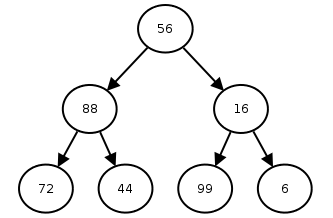
\includegraphics[scale=0.9]{obrazky/3BinarniStrom.png}
	\caption{Binární strom}
\end{figure}

\medskip
\subsection{Binární vyhledávací strom}
Binární \textit{vyhledávací} strom (zkratka BVS), je speciální typ binárního stromu, kde platí následující:
\begin{itemize}
\item \textbf {Každý \textit{pravý} potomek $P$ rodiče $R$ má vyšší hodnotu $h$ než jeho rodič.} Platí tedy: $P.h > R.h$ $\Rightarrow$ Pravý podstrom uzlu $R$, obsahuje pouze uzly, které mají vyšší hodnotu než uzel $R$. 
\item \textbf {Každý \textit{levý} potomek $L$ rodiče $R$ má nižší hodnotu $h$ než jeho rodič.} Platí tedy: $P.h > L.h$ $\Rightarrow$ Levý podstrom uzlu $R$, obsahuje pouze uzly, které mají nižší hodnotu než uzel $R$. 
\item \textbf {Ve stromě se nenachází dva uzly se stejnou hodnotou.}
\end{itemize} 

\noindent Toto uspořádání uzlů v BVS usnadňuje vyhledávání. Operace nad BVS stromem s výškou \textit{v}  mají časovou složitost $ \theta$(\textit{v}). V nejhorším případě může mít BVS výšku rovnu \textit{n} - 1, kde \textit{n} je počet uzlů. Oba případy jsou zobrazeny na obrázku \ref{binary}.

\begin{figure}[h!]
\centering
	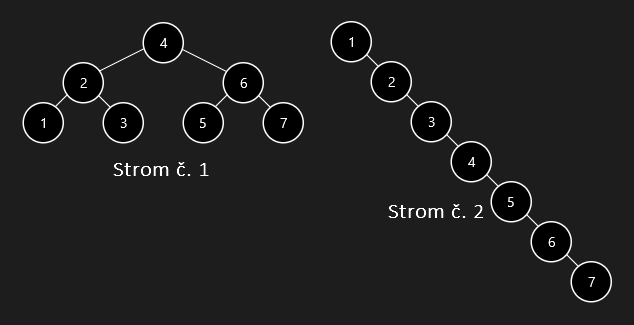
\includegraphics[scale=0.7]{obrazky/4BinarniVyhledavaciStrom.png}
	\caption{Rozdílné výšky stromu}
	\label{binary}
\end{figure}

\subsubsection{Vyhledávání}
Operace \textit{vyhledávání} patří k nejčastěji používané operaci s BVS. Při \textit{vyhledávání} je potřeba zadat hodnotu $x$, kterou chceme vyhledat. Postupně dochází k porovnávání hodnot uzlů s $x$. Výsledkem vyhledávání je buď uzel, který obsahuje hodnotu $x$ nebo takový uzel neexistuje.\\

\noindent \textbf{Přesný postup vyhledávání:}
\begin{enumerate} {\bfseries
\item  krok} -- počáteční \\
Na začátku vyhledávání je třeba určit aktuální uzel, který označíme $u$. Hledanou hodnotu označíme $x$.\\
V tomto kroku $u$ bude kořen stromu, pokud strom nemá kořen hodnota $x$ je nenalezena a tím vyhledávání končí.
{\bfseries\item  krok} -- průběžný \\
Zde dochází k porovnávání $x$ a hodnoty aktuálního uzlu $u$. Hodnotu $u$ označíme $u.h$.\\
Pokud je $u$ prázdný vyhledávání končí neúspěchem. \\\\
\textbf{Při porovnávání mohou nastat tyto možnosti:}
\begin{itemize}
\item $x > u.h$ \\
V tomto případě jako $u$ nastavíme pravého potomka $u$. A znovu provedeme 2. krok.
\newpage
\item $x < u.h$\\
V tomto případě jako $u$ nastavíme levého potomka $u$. A znovu provedeme 2. krok.
\item $x = u.h$\\
Hledaná hodnota $x$ byla nalezena v $u$. Vyhledávání tedy končí.
\end{itemize}
\end{enumerate}

\medskip
\noindent Na obrázku \ref{binarySearch} je zvýrazněna cesta průchodů stromem při vyhledávání uzlu s hodnotou 5. V obrázku je i zaznamenána historie porovnávání. 

\begin{figure}[h!]
\centering
	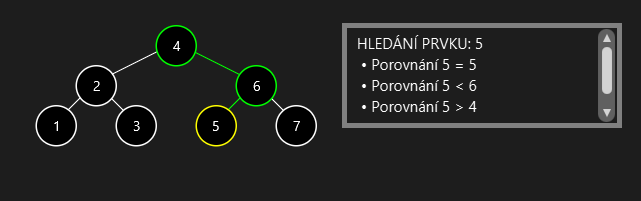
\includegraphics[scale=0.9]{obrazky/5BinarniVyhledavani.png}
	\caption{Vyhledávání hodnoty 5}
	\label{binarySearch}
\end{figure}

\medskip \medskip \medskip
\noindent \textbf{Zdrojový kód vyhledávání v jazyku Java:}

\begin{kicode}{Java}{search}
Node search(int value, Node node) { //value je hledaná hodnota, node je při prvním volání kořen
	if (node == null) {
		return null; //uzel nebyl nalezen
	}
	
	if (value > node.getValue()) { //pokud je hledaná hodnota je vyšší než má aktuální uzel
		search(value, node.getRight()); //nastavím aktuální uzel na pravého potomka
	} else if (value < node.getValue()) { //pokud je hledaná hodnota je vyšší než má aktuální uzel
		search(value, node.getLeft()); //nastavím aktuální uzel na levého potomka
	} else { //pokud není vyšší ani nižší, tak se musí rovnat
		return node; //vrátím nalezený uzel
	}
}
\end{kicode}

\newpage
\subsubsection{Vkládání}
Při \textit{vkládání} zadané hodnoty $x$ je nejprve nutné prohledat strom, jestli se zde $x$ již nenachází. Pokud je nalezen uzel s hodnotou $x$, je výsledkem operace nalezený uzel. V případě, že daný strom tento uzel neobsahuje, je jako potomek posledního prohledávaného uzlu vložen nový uzel s hodnotou $x$. \\


\noindent \textbf{Přesný postup vkládání:}
\begin{enumerate} {\bfseries
\item  krok} -- počáteční \\
Na začátku vkládání je třeba určit aktuální uzel, který označíme $u$. Vkládanou hodnotu označíme $x$.\\
V tomto kroku $u$ bude kořen stromu. Pokud strom nemá kořen vytvoříme nový uzel s hodnotou $x$ a vložíme do stromu. Uzel se stane kořenem stromu, čímž vkládání končí.
{\bfseries\item  krok} -- vyhledávání, vkládání \\
Před vkládáním je nejprve nutno ověřit, zde se ve stromu nenachází uzel s hodnotou $x$.\\\\
\textbf{Vyhledávání může dopadnou těmito způsoby:}
\begin{itemize}
\item Prvek byl nalezen. \\
Pokud byl uzel s hodnotou $x$ nalezen, vkládání končí neúspěchem.
\item Prvek nebyl nalezen, přičemž platí $x > u.h$\footnote{\label{hodnotaPosledniho}Hodnota posledního navštíveného uzlu, při hledání}.\\
Vytvoříme nový uzel s hodnotou $x$ a vložíme ho jako pravého potomka $u$\footnote{\label{posledni}Poslední navštívený uzel, při hledání.}
\item Prvek nebyl nalezen, přičemž platí $x < u.h$\footnoteref{hodnotaPosledniho}.\\
Vytvoříme nový uzel s hodnotou $x$ a vložíme ho jako pravého potomka $u$\footnoteref{posledni}
\end{itemize}
\end{enumerate}

\medskip
\noindent Na obrázku \ref{binarySearchInsert} je zvýrazněna cesta průchodů stromem při vyhledávání uzlu s hodnotou 6. Samotné vložení je na obrázku \ref{binaryInsert}.

\begin{figure}[h!]
\centering
	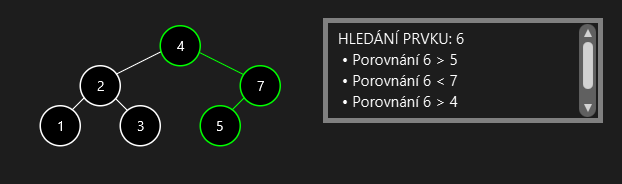
\includegraphics[scale=0.9]{obrazky/6BinarniVkladani1.png}
	\caption{Vkládání hodnoty 6 - hledání}
	\label{binarySearchInsert}
\end{figure}

\begin{figure}[h!]
\centering
	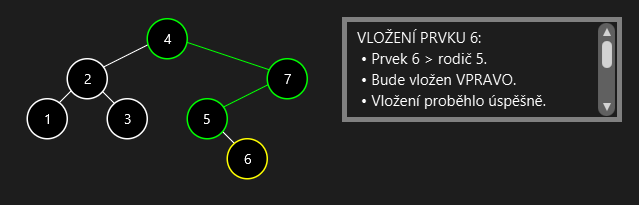
\includegraphics[scale=0.9]{obrazky/6BinarniVkladani2.png}
	\caption{Vkládání hodnoty 6 - vložení}
	\label{binaryInsert}
\end{figure}

\newpage
\noindent \textbf{Zdrojový kód vkládání v jazyku Java:}\\\\
\noindent Před samotnou funkcí \kiinlinecode{Java}{!}{insert} je třeba vytvořit třídu \kiinlinecode{Java}{!}{Result}, která bude dále použita:
\begin{kicode}{Java}{Class Result}
Class Result() {
	private Node node; //poslední navštívený uzel (hledaný/rodič)
	private boolean isFind; //parametr pro určení zda byl uzel nalezen
	
	public Result(Node node, boolean isFind) { //konstruktor
		...
	}	
	...
}
\end{kicode}

\noindent Dále je potřeba trochu poupravit již známou funkci \kiinlinecode{Java}{!}{search} je třeba vytvořit třídu \kiinlinecode{Java}{!}{Result}, která bude dále použita:


%% Závěry práce. V jazyce práce a anglicky. Text pro jiný než
%% nastavený jazyk práce (nepovinným parametrem language makra
%% \documentclass, výchozí český) se zadává použitím makra s uvedením
%% jazyka jako nepovinného parametru.
\begin{kiconclusions}
Závěr práce v \uv{českém} jazyce.
\end{kiconclusions}

\begin{kiconclusions}[english]
Thesis conclusions in \uv{English}.
\end{kiconclusions}

%% Přílohy obsahu textu práce, za makrem \appendix.
\appendix

\section{První příloha}
Text první přílohy

\section{Druhá příloha}
Text druhé přílohy

%% Obsah přiloženého CD/DVD. Poslední příloha. Upravte podle vlastní
%% práce!
\section{Obsah přiloženého CD/DVD} \label{sec:ObsahCD}

Na samotném konci textu práce je uveden stručný popis obsahu
přiloženého CD/DVD, tj.~jeho závazné adresářové struktury, důležitých
souborů apod.

\begin{description}

\item[\texttt{bin/}] \hfill \\
  Instalátor \textsc{Instalator} programu, popř.~program
  \textsc{Program}, spustitelné přímo z~CD/DVD. / Kompletní adresářová
  struktura webové aplikace \textsc{Webovka} (v~ZIP archivu) pro
  zkopírování na webový server. Adresář obsahuje i~všechny runtime
  knihovny a~další soubory potřebné pro bezproblémový běh instalátoru
  a~programu z~CD/DVD / pro bezproblémový provoz webové aplikace na
  webovém serveru.

\item[\texttt{doc/}] \hfill \\
  Text práce ve formátu PDF, vytvořený s~použitím závazného stylu KI
  PřF UP v~Olomouci pro závěrečné práce, včetně všech příloh,
  a~všechny soubory potřebné pro bezproblémové vygenerování PDF
  dokumentu textu (v~ZIP archivu), tj.~zdrojový text textu, vložené
  obrázky, apod.

\item[\texttt{src/}] \hfill \\
  Kompletní zdrojové texty programu \textsc{Program} / webové aplikace
  \textsc{Webovka} se všemi potřebnými (příp.~převzatými) zdrojovými
  texty, knihovnami a~dalšími soubory potřebnými pro bezproblémové
  vytvoření spustitelných verzí programu / adresářové struktury pro
  zkopírování na webový server.

\item[\texttt{readme.txt}] \hfill \\
  Instrukce pro instalaci a~spuštění programu \textsc{Program}, včetně
  všech požadavků pro jeho bezproblémový provoz. / Instrukce pro
  nasazení webové aplikace \textsc{Webovka} na webový server, včetně
  všech požadavků pro její bezproblémový provoz, a~webová adresa, na
  které je aplikace nasazena pro účel testování při tvorbě posudků
  práce a~pro účel obhajoby práce.

\end{description}

Navíc CD/DVD obsahuje:

\begin{description}

\item[\texttt{data/}] \hfill \\
  Ukázková a~testovací data použitá v~práci a~pro potřeby testování
  práce při tvorbě posudků a~obhajoby práce.

\item[\texttt{install/}] \hfill \\
  Instalátory aplikací, runtime knihoven a~jiných souborů potřebných
  pro provoz programu \textsc{Program} / webové aplikace
  \textsc{Webovka}, které nejsou standardní součástí operačního
  systému určeného pro běh programu / provoz webové aplikace.

\item[\texttt{literature/}] \hfill \\
  Vybrané položky bibliografie, příp.~jiná užitečná literatura
  vztahující se k~práci.

\end{description}

U~veškerých cizích převzatých materiálů obsažených na CD/DVD jejich
zahrnutí dovolují podmínky pro jejich šíření nebo přiložený souhlas
držitele copyrightu. Pro všechny použité (a~citované) materiály,
u~kterých toto není splněno a~nejsou tak obsaženy na CD/DVD, je uveden
jejich zdroj (např.~webová adresa) v~bibliografii nebo textu práce
nebo v souboru \texttt{readme.txt}.

%% -------------------------------------------------------------------

%% Sazba volitelného seznamu zkratek, za přílohami.
%\printglossary

%% Sazba povinné bibliografie, za přílohami (případně i za seznamem
%% zkratek). Při použití BibLaTeXu použijte makro
%% \printbibliography. jinak prostředí thebibliography. Ne obojí!

%% Sazba i v textu necitovaných zdrojů, při použití
%% BibLaTeXu. Volitelné.
\nocite{*}
%% Vlastní sazba bibliografie při použití BibLaTeXu.
%% \printbibliography


\newpage


\begin{thebibliography}{99}	

\bibitem{belohlavekALM} \uppercase{BĚlohlávek}, Radim. Algoritmická matematika 2 - část 1 [online]. 2012-05-15. [cit. 2018-07-07]. Dostupné z: \url{http://belohlavek.inf.upol.cz/vyuka/algoritmicka-matematika-2-1.pdf}

\bibitem{belohlavekVychodil} \uppercase{BĚlohlávek}, Radim; \uppercase{Vychodil}, Vilém; Diskrétní matematika pro informatiky II [online]. 2010-10-16. [cit. 2018-07-07]. Dostupné z: \url{http://belohlavek.inf.upol.cz/vyuka/dm2.pdf}

\bibitem{dvorsky} \uppercase{DvorskÝ}, Jiří. Algoritmy I.[online]. 2007-02-27. [cit. 2018-07-07]. Dostupné z: \url{http://www.cs.vsb.cz/dvorsky/Download/SkriptaAlgoritmy/Algoritmy.pdf}

\bibitem{BinarySearch} \uppercase{Binary Search Trees}
Dostupné z: \url{http://cs.umw.edu/~finlayson/class/fall12/cpsc230/notes/17-binary-search-trees.html}

\end{thebibliography}
%% Bibliografie, včetně sazby, při nepoužití BibLaTeXu.
% \begin{thebibliography}{9}
%\bibitem{kniha2} \uppercase{Hawke}, Paul. NanoHttpd: Light-weight HTTP server designed for embedding in other applications. GitHub [online]. 2014-05-12. [cit. 2014-12-06]. Dostupné z: \url{https://github.com/NanoHttpd/nanohttpd}
%
%\bibitem{jeske13} \uppercase{Jeske}, David; \uppercase{Novák}, Josef. Simple HTTP Server in \csharp: Threaded synchronous HTTP Server abstract class, to respond to HTTP requests. CodeProject: For those who code [online]. 2014-05-24. [cit. 2014-12-06]. Dostupné z: \url{http://www.codeproject.com/Articles/137979/Simple-HTTP-Server-in-C}
%
%\bibitem{uzis2012} \uppercase{ÚSTAV ZDRAVOTNICKÝCH INFORMACÍ A STATISTIKY ČR}. Lékaři, zubní lékaři a farmaceuti 2012 [online]. Praha 2, Palackého náměstí 4: Ústav zdravotnických informací a statistiky ČR, 2012 [cit. 2014-12-06]. ISBN 978-80-7472-089-5. Dostupné z: \url{http://www.uzis.cz/publikace/lekari-zubni-lekari-farmaceuti-2012}



%% Sazba volitelného rejstříku, za bibliografií.
\printindex

\end{document}
